% !TEX root = 4268671_Janik_Frick_T1000.tex
\section{Parametertabellenkonfigurator}
Mit Hilfe des \glqq Parametertabellenkonfigurators\grqq\space sollen die Installationsabläufe von Programmen und Produkten von Blum auf CNC-Maschinen unterstützt werden.
\subsection{Problemstellung}
Bei bestehenden Programmen für numerische Steuerungen müssen während der Inbetriebnahme Parametertabellen in einem beliebigen Texteditor angepasst werden. Aufgrund der Anzahl, wie auch der Einstellmöglichkeiten der Parameter, zu sehen in Abbildung \ref{fig:Paratab}, wird hierfür eine separate Installationsanleitung benötigt. Der Prozess der Parametrierung ist daher Fehleranfällig und von der Erfahrung des Inbetriebnehmers abhängig. Um den hohen Anforderungen der Kunden gerecht zu werden, gilt es potenzielle Fehlerquellen zu eliminieren. Hierfür soll selbstständig ein \glqq Parametertabellenkonfigurator\grqq\space entwickelt werden.
\begin{figure}[H]
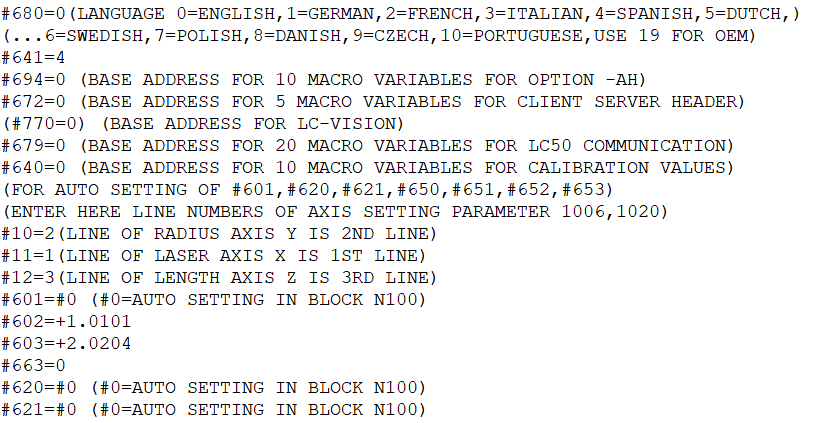
\includegraphics[scale=0.7]{pictures_and_research/Bilder/Paratab.PNG}
\caption{Auszug einer Parametertabelle}
\label{fig:Paratab}
\end{figure}
\subsection{Anforderungen}
\label{Anfs} 
An den \glqq Parametertabellenkonfigurator\grqq\space gibt es mehrere Anforderungen. \\
Parametertabellen sollen eingelesen und angezeigt werden können. Zu den Parametern soll es ermöglicht werden, Beschreibungen aus Text und Bild speichern und anzeigen zu können.\\
Diese Anforderungen sind aus dem Bereich der funktionalen Anforderungen (\ref{Anforderungstypen}).\\
Nicht funktionale Anforderungen (\ref{Anforderungstypen}) sind die Verwendung der Programmiersprache und das Verwenden des in C++ entwickelten Framework Qt.\\
Aus diesen Anforderungen lässt sich ableiten, welche \ac{GUI}-Elemente nötig sind und welche Funktionalitäten benötigt werden.\\
Um die Anforderungen an den \glqq Parametertabellenkonfigurator\grqq\space zu sammeln, die nicht im Auftragsdokument stehen, wurde das Interview (\ref{interview}) gewählt. Die Entscheidung wurde getroffen, weil in offenen Gesprächen mehr Zusatzinformationen fließen, als in Umfragen (\ref{Fragebögen}) oder durch Beobachtung (\ref{Beobachtung}). Zusätzlich kann auf Verständnisschwierigkeiten reagiert werden, solange das Gespräch noch aktuell ist und der Kontext noch nicht vergessen ist.\\
Hauptergebnis ist die Erstellung einer übersichtlichen \ac{GUI}.\\
Die Anforderungen zielen darauf ab, ein \ac{MVP} zu erstellen. Ein \ac{MVP} erfüllt die wichtigsten Anforderungen an das Produkt, ist aber noch nicht so weit entwickelt, dass es alle für den Einsatz notwendigen Anforderungen erfüllt.
\subsubsection{Notwendige Funktionalitäten}
Um die Parametertabellen anzeigen zu können, müssen diese aus einer Datei eingelesen werden. Um Konfigurationen festzuhalten, wird eine Funktion zum Speichern der Tabellen benötigt. \\
Für die Beschreibungen wird zusätzlich eine Funktion benötigt um diese mit den richtigen Parametern zu verknüpfen. \\
\subsubsection{Notwendige GUI-Elemente}
Die \ac{GUI} benötigt Anzeigemöglichkeiten für die Parametertabellen und Beschreibungen, Angaben von Namen, Steuerung und Produkttyp zur aktuellen Parametertabelle und den aktuellen Parameter.\\
Für die Bedienung der Anzeigeelemente werden Steuerelemente für das Laden und Bearbeiten von Parametertabellen und Beschreibungen benötigt.
\subsection{GUI-Entwurf}
Um die \ac{GUI} zu entwerfen, kommt ein Prototyp (\ref{Prototypen}) zum Einsatz, der mit dem Mockup-Tool "Balsamiq Mockup 3\grqq\space erstellt wurde. Das Tool bietet nahezu alle gängigen \ac{GUI}-Elemente an und kann diese miteinander verknüpfen, so dass schon in einem frühen Stadium Abläufe nachvollzogen und besprochen werden können. Zusätzlich bietet das Tool eine unkomplizierte Möglichkeit, alternative Entwürfe zu entwerfen und in den Ablauf der Simulation zu integrieren. Das unterstützt den Prozess während der Entwicklung der \ac{GUI}, da neue Vorschläge in kurzer Zeit besprochen und weiterentwickelt werden können.\\
\newline
Die \ac{GUI} ist aus mehreren einzelnen Fenstern aufgebaut. Dieser Aufbau unterstützt die Übersichtlichkeit und der Benutzerführung bei der Verwendung, da jeweils nur die benötigten Informationen und Funktionen angezeigt werden.\\ 
Insgesamt besteht die \ac{GUI} aus vier Fenstern, die dem Benutzer die benötigten Funktionen zur Verfügung stellen. \\
Das in Abbildung \ref{fig:filep} dargestellte Fenster dient dem Zweck bei erster Benutzung den Pfad zu einer Datenbank einzugeben, in der die Beschreibungen gespeichert sind. Im nächsten Fenster, zu sehen in Abbildung \ref{fig:filepError}, lässt sich die Auswahl der Parametertabellen konfigurieren. Nach der Auswahl einer Parametertabelle wird diese im Hauptfenster, siehe Abbildung \ref{fig:ConfigW}, angezeigt. In diesem Fenster werden die Beschreibungen der Parameter angezeigt und die Parametertabelle kann angepasst werden. Es gibt Steuerelemente für die Navigation durch die Parametertabelle, für die Navigation durch die Fenster und die Möglichkeit die geänderte Parametertabelle zu speichern.\\
\begin{figure}[H]
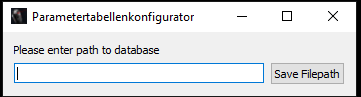
\includegraphics[scale=1]{pictures_and_research/Bilder/filepathWindow.PNG}
\caption{Fenster um den Dateipfad der Datenbank einzugeben,\\
es gibt einen Standardpfad}
\label{fig:filep}
\end{figure}
\begin{figure}[H]
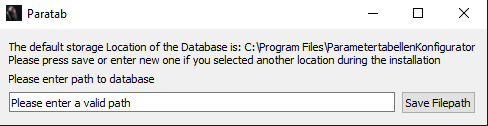
\includegraphics[scale=1]{pictures_and_research/Bilder/errorFilePathW.PNG}
\caption{Wurde ein nicht vorhandener Pfad eingegeben erscheint die Fehlermeldung "Please enter a valid path"}
\label{fig:filepError}
\end{figure}
\begin{figure}[H]
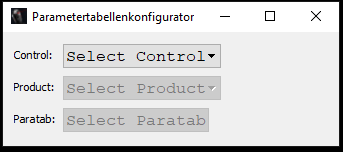
\includegraphics[scale=1]{pictures_and_research/Bilder/configW.PNG}
\caption{Fenster um Auswahl der Parametertabellen zu konfigurieren}
\label{fig:ConfigW}
\end{figure}
\begin{figure}[H]
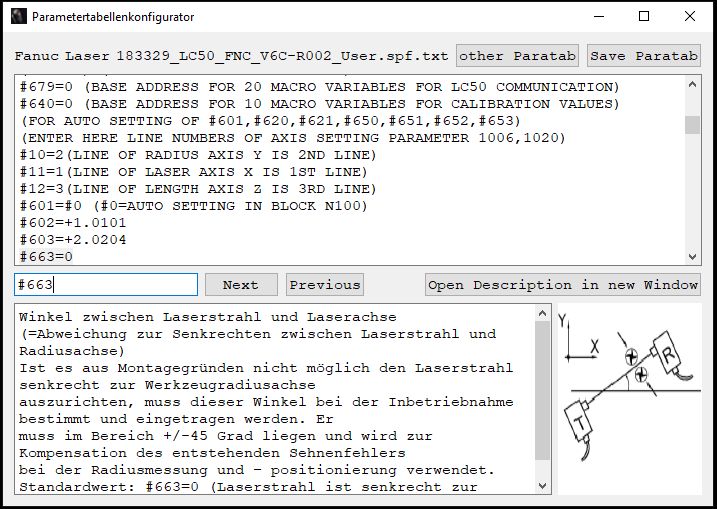
\includegraphics[scale=0.75]{pictures_and_research/Bilder/paratabW.PNG}
\caption{Fenster für die Anzeige der Parametertabellen und deren Beschreibungen}
\label{fig:Paraw}
\end{figure}
\noindent
In Abbildung \ref{fig:Paraw} werden im oberen Bereich Informationen zur aktuell ausgewählten Parametertabelle angezeigt. Oben rechts gibt es Steuerelemente, um eine andere Parametertabelle auszuwählen, oder um die Aktuelle zu speichern.\\
Unterhalb der Anzeige für die Parametertabelle ist der Bereich für detaillierte Informationen zum aktuellen Parameter. Es gibt Steuerelemente, um andere Parameter auszuwählen. Dies ist mit den Buttons \glqq Next\grqq\space und \glqq Previous\grqq\space möglich, die jeweils um einen Parameter nach oben oder nach unten springen. Durch direkte Eingabe eines Parameters in das Parameterfeld kann zu einem beliebigen Parameter gesprungen werden. Um größere Beschreibungen übersichtlich sehen zu können, gibt es die Möglichkeit die Beschreibung isoliert in einem neuen Fenster zu öffnen.\\
\begin{figure}[H]
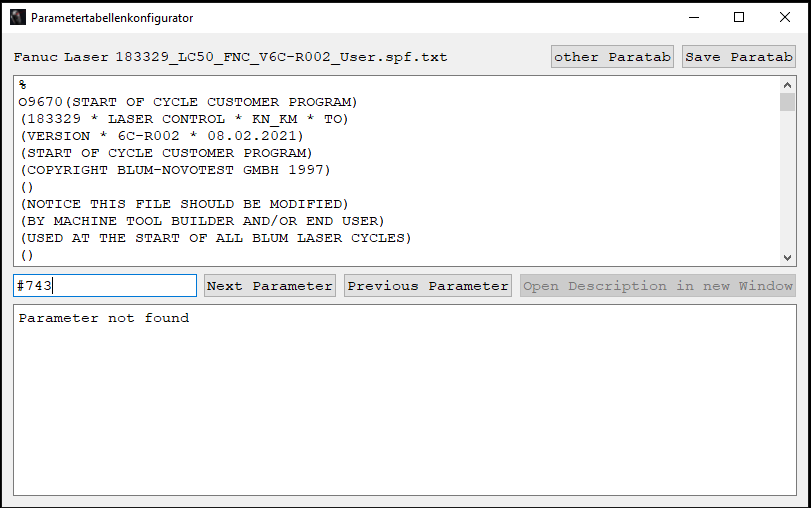
\includegraphics[scale=0.6]{pictures_and_research/Bilder/fehlermeldung_invalid_parameter.PNG}
\caption{Wird ein nicht vorhandener Parameter in das Feld eingegeben wird eine Fehlermeldung angezeigt.}
\label{fig:paraError}
\end{figure}
\begin{figure}[H]
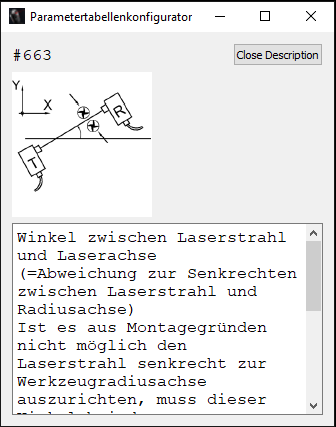
\includegraphics[scale=1]{pictures_and_research/Bilder/descriptW.PNG}
\caption{Isolierte Ansicht einer Beschreibung eines Parameters}
\label{fig:descript}
\end{figure}\noindent
Das in Abbildung \ref{fig:descript} sichtbare Bild der Beschreibung hat eine konstante Größe. Der Grund dafür ist, dass ansonsten bei Änderung der Fenstergröße das Bild verzerrt werden würde und das Erkennen von wichtigen Informationen im Bild erschwert werden würde.
\subsection{Programmierung}
Für die Programmierung wird wie in den nicht funktionalen Anforderungen (\ref{Anfs}) vorgegeben C++ mit dem für \ac{GUI} optimierten Framework Qt verwendet. \\
Da Qt für den Aufbau von Benutzeroberflächen Klassen bereitstellt, wird die Software objektorientiert (\ref{Objektorientierung}) programmiert. Um den Code auch mit wachsender Größe lesbar und verständlich zu halten, kommen \lq Clean-Code Prinzipien\rq\space(\ref{CC}) zum Einsatz.\\
\subsubsection{Softwarestruktur}
Um die Software flexibel zu gestalten, wird diese mit Hilfe von modular programmiert. Die Modularität wird durch die Projektorientierte Programmierung (\ref{Objektorientierung}) unterstützt. Die Logik und die \ac{GUI} bestehen aus mehreren einzelnen Klassen, die als Module betrachtet werden können. Um die einzelnen Module zu verbinden, gibt es eine \lq Managerklasse\rq\space für den Logikteil und eine für die Module der \ac{GUI}. Um diese beiden \lq Managerklassen\rq\space ebenfalls unabhängig zu halten, gibt es eine weitere \lq Managerklasse\rq\space die dafür verantwortlich ist, die Daten zwischen Logik und \ac{GUI} zu transferieren. \\
Diese Trennung, erkennbar in Abbildung \ref{fig:UML}, ermöglicht es Anpassungen an den einzelnen Modulen vorzunehmen, ohne die höheren Ebenen grundlegend anzupassen.
\begin{figure}[H]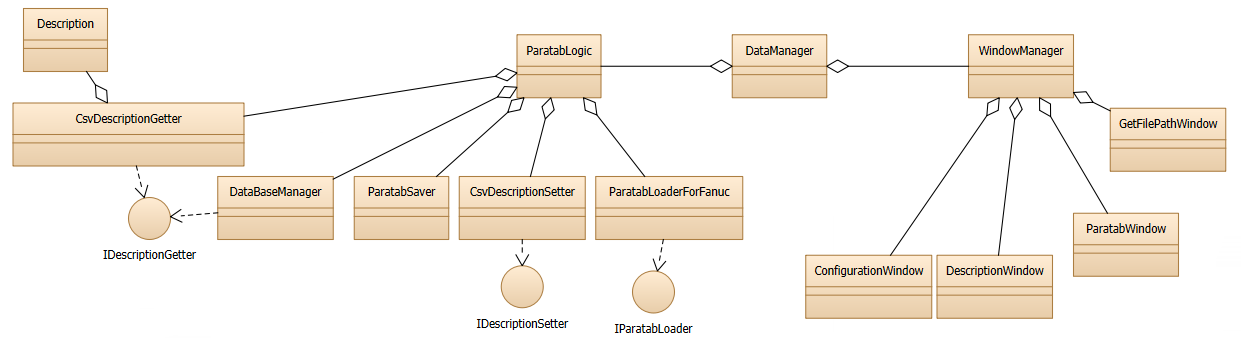
\includegraphics[page=1,scale=0.49]{pictures_and_research/Bilder/uml.PNG}
\caption{\ac{UML}-Diagramm der Software ohne attribute der Klassen}
\label{fig:UML}
\end{figure}\noindent
Das Diagramm in Abbildung \ref{fig:UML} dient dazu die Modularität der Software zu veranschaulichen, daher wurde auf die Darstellung von Inhalten der Klassen verzichtet.\\
\ac{UML} dient dazu, die Architektur von Software zu visualisieren. Klassen werden durch Rechtecke visualisiert, Interfaces durch Kreise. Pfeile mit gestrichelten Strichen symbolisieren Vererbung. Von dem Element, auf das der Pfeil zeigt, werden Attribute geerbt.s\subsubsection{Verarbeitung von Benutzeraktionen}
Interagiert der Benutzer mit der \ac{GUI} werden entsprechende Veränderungen erwartet. \\
Qt bietet für die Verarbeitung der Benutzeraktionen mit dem \lq Signal-Slot Mechanismus\rq\space Unterstützung. Dieser Mechanismus bietet die Möglichkeit Signale auszusenden, die von einem verbundenen Slot empfangen werden können. Dabei muss das Senderobjekt keine Verbindung zum Empfängerobjekt haben. Die Verbindung zwischen Signal kann entweder direkt im Empfängerobjekt, oder in einer Instanz einer \lq Managerklasse\rq\space eingerichtet werden. Grundvoraussetzung ist, dass das Objekt, in dem die Verbindung eingerichtet ist, sowohl eine Verbindung mit dem Sender- als auch mit dem Empfängerobjekt hat.\\
Die meisten Klassen die von Qt bereitgestellt werden, haben vordefinierte Signale. Diese erlauben es die Benutzerinteraktionen zu verarbeiten und entsprechend darauf zu reagieren. \\
Neben den vordefinierten Signalen von \ac{GUI}-Elementen können auch selbst definierte Signale eingesetzt werden, um Methoden aufzurufen. Signale von \ac{GUI}-Elementen werden ohne weitere Implementierungen durch den Entwickler gesendet. Selbst definierte Signale müssen mit einem Befehl gesendet werden. Signale können auch Daten übergeben, die vom verbundenen Slot verarbeitet werden können. Dabei muss die Zahl der Argumente des Slots nicht mit der des Signals übereinstimmen. Signale können mit allen Slots verbunden werden, die gleich viele oder weniger Argumente entgegennehmen. Begrenzend wirkt hier die Reihenfolge der Datentypen der Argumente. Diese muss übereinstimmen.\\
Dieser Mechanismus ermöglicht weitere Flexibilität, da jederzeit neue Verbindungen erstellt werden können, oder bestehende entfernt werden können. Diese Funktionalität ist hilfreich, wenn das Ausführen einer Methode Signale aussenden würde, die unerwünschte Folgen hätten. In diesem Fall kann man die Verbindung von Signal und Slot zu Beginn der Methode trennen und am Ende der Methode wieder herstellen. \\
\subsubsection{Speicherung der Beschreibungen}
Die Beschreibungen der Parameter werden in einer relationalen Datenbank gespeichert. Relationale Datenbanken speichern Daten in Tabellen, in denen eine Spalte als eindeutiger Schlüssel , \lq Primary Key\rq\space für die Reihen dient. Relationen zwischen Elementen werden durch eine zusätzliche Spalte symbolisiert. In dieser Spalte wird der \lq Primary Key\rq\space der Reihe eingetragen, zu der eine Verbindung besteht. Es ist nicht relevant, ob die verbundene Reihe in der selben oder einer anderen Tabelle steht. In relationalen Datenbanken werden werden die Daten nicht über die Position, sondern über den \lq Primary Key\rq\space direkt adressiert. Die genaue Position der Objekte in der Datenbank ist nicht bekannt\cite{10.1145/1283920.1283937}.\\
Der Grund für die Wahl dieses Models wurde getroffen, da Beschreibungen und Bilder eindeutig einem Parameter zugeordnet werden können. Da der Parameter, für den die Beschreibung geladen werden soll, bekannt ist, ist der fehlende Zugriff über die Position kein Hindernis.
\subsubsection{Tests}
Die Software wird abgesehen von der GitLab Pipeline (\ref{Tools}) manuell getestet. Dies hat den Grund, dass die Automatisierung von Tests anspruchsvoll und zeitaufwendig ist (\ref{Tests}).
\subsubsection{Verwendete Tools}
\label{Tools}
Um die Entwicklung zu unterstützen werden Tools für die Versionsverwaltung und \lq Continous Developement/ Integration\rq\space (\ref{CI}) eingesetzt.\\
Für die Versionsverwaltung kommen GitKraken und GitLab zum Einsatz. GitKraken dient als Schnittstelle zwischen dem lokalen Projekt auf dem Computer und der Plattform für \lq Continous Developement/ Integration\rq\space \ref{CI} GitLab. In GitKraken lässt sich der gesamte Verlauf des Projekts einsehen. Außerdem können alte Commits \ref{Git} ausgewählt werden und direkt in einer Entwicklungsumgebung geöffnet werden. Für die Sicherung auf dem Server bietet GitKraken die Git Befehle, die durch eine graphische Benutzeroberfläche oder durch das integrierte Terminal genutzt werden können.\\
GitLab wird nicht nur für die Sicherung von Softwareständen auf einem Server eingesetzt. Ebenfalls genutzt werden die Möglichkeiten für das Organisieren von To-Do's durch \lq Issues\rq ,\space sowie die GitLab Pipeline. Die GitLab Pipeline ist ein Feature im Kontext von Continous Integration \ref{CI}. Zusätzlich werden während dem Prozess Artefakte erstellt, in denen Dateien gesammelt werden, die für das Erstellen eines Installers benötigt werden. Diese Artefakte lassen sich nach dem erfolgreichen Durchlauf der Pipeline als ZIP-Ordner herunterladen.\\ 
\subsection{Anwendung der Software}
Vor der Bearbeitung wird im ConfigurationWindow, Abbildung 3, die Steuerung und das Produkt festgelegt. Durch klicken auf \glqq Select Paratab\grqq\space wird ein Dateiexplorer-Fenster geöffnet. Durch die getroffene Auswahl im ConfigurationWindow, Abbildung 3, werden die angezeigten Dateien im Dateiexplorer gefiltert um die Auswahl der richtigen Parametertabelle zu vereinfachen. Die ausgewählte Parametertabelle wird im ParatabWindow, Abbildung 4 und 5, angezeigt.\\
Um einen Parameter zu bearbeiten, muss die entsprechende Zeile im Textfeld ausgewählt zu werden. Dazu gibt es unterschiedliche Möglichkeiten. Man kann eine Zeile direkt durch anklicken mit der Maus auswählen. Möchte der Benutzer jeden Parameter nacheinander konfigurieren bieten die Buttons \lq Next\rq\space und \lq Previous\rq\space die Möglichkeit direkt zum nächsten, beziehungsweise zum vorherigen Parameter zu springen, ohne danach zu suchen. Geht es darum bestimmte Parameter an verschiedenen Stellen zu bearbeiten, kann im Feld für die Anzeige des aktuellen Parameters ein Parameter eingegeben werden. Ist der eingegebene Parameter in der Tabelle enthalten, springt die Anzeige direkt zu diesem Parameter.\\
Um zu prüfen, ob eine Zeile einen Parameter enthält kommen \lq Reguläre Ausdrücke\rq\space zum Einsatz. Mit Diesen lassen sich Texte auf bestimmte Inhalte oder Muster untersuchen. \\
In dieser Software wird mit Hilfe der Cursor-Klasse von Qt die gesamte Zeile ausgewählt und mit einem \lq Regulären Ausdruck\rq\space untersucht. \\
Um die Bearbeitung der Parameter zu unterstützen wird unterhalb der Anzeige für die Parametertabelle die Beschreibung des Parameters angezeigt. Die Option \glqq Open Description in new Window\grqq ,\space Abbildung 4 und 5, hilft bei langen Beschreibungstexten und Bildern das Lesen der Beschreibung zu vereinfachen. Es öffnet sich ein neues Fenster, zu sehen in Abbildung 6, in dem die Beschreibung und das Bild isoliert angezeigt werden.\\
Ist die Konfiguration der Parametertabelle abgeschlossen, kann in der oberen rechten Ecke, zu sehen in Abbildung 4 und 5, die Parametertabelle gespeichert werden. 